\begin{visualexample}
\begin{figure}[H]
    \centering
    % Step 1: Show all points, highlight p0
    \begin{subfigure}{0.32\textwidth}
        \centering
        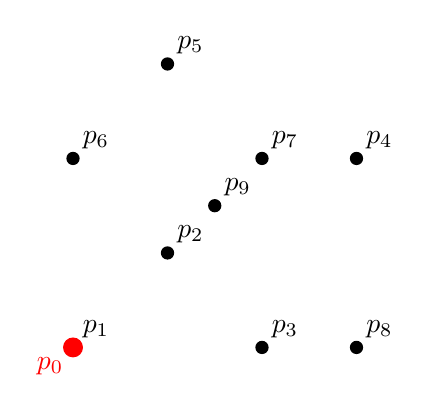
\begin{tikzpicture}[scale=1.2]
            % Points
            \foreach \x/\y/\n in {1/1/1, 2/2/2, 3/1/3, 4/3/4, 2/4/5, 1/3/6, 3/3/7, 4/1/8, 2.5/2.5/9} {
                \fill (\x,\y) circle (2pt);
                \node[above right] at (\x,\y) {$p_{\n}$};
            }
            % Highlight p0
            \fill[red] (1,1) circle (3pt);
            \node[below left, red] at (1,1) {$p_0$};
        \end{tikzpicture}
        \caption{Step 1: Highlight $p_0$ (bottom-most point)}
    \end{subfigure}
    % Step 2: Show rays from p0 to all other points
    \begin{subfigure}{0.32\textwidth}
        \centering
        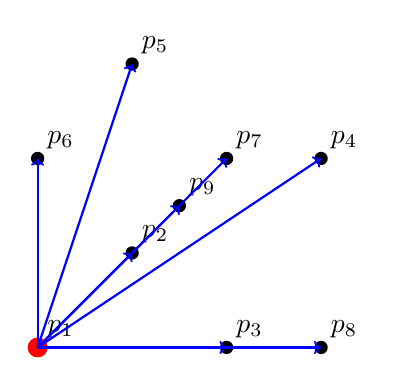
\begin{tikzpicture}[scale=1.2]
            % Points
            \foreach \x/\y/\n in {1/1/1, 2/2/2, 3/1/3, 4/3/4, 2/4/5, 1/3/6, 3/3/7, 4/1/8, 2.5/2.5/9} {
                \fill (\x,\y) circle (2pt);
                \node[above right] at (\x,\y) {$p_{\n}$};
            }
            % Highlight p0
            \fill[red] (1,1) circle (3pt);
            % Rays
            \foreach \x/\y in {2/2, 3/1, 4/3, 2/4, 1/3, 3/3, 4/1, 2.5/2.5} {
                \draw[->, blue, thick] (1,1) -- (\x,\y);
            }
        \end{tikzpicture}
        \caption{Step 2: Draw rays from $p_0$ to all other points}
    \end{subfigure}
    % Step 3: Show sorted order (by numbering or arrows)
    \begin{subfigure}{0.32\textwidth}
        \centering
        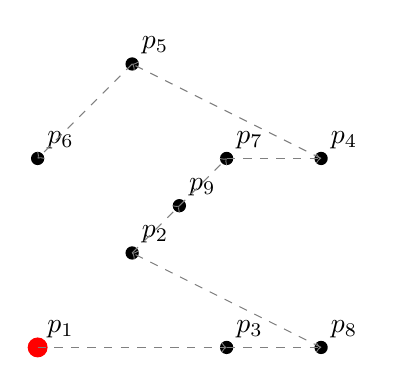
\begin{tikzpicture}[scale=1.2]
            % Points
            \foreach \x/\y/\n in {1/1/1, 3/1/3, 4/1/8, 2/2/2, 2.5/2.5/9, 3/3/7, 4/3/4, 2/4/5, 1/3/6} {
                \fill (\x,\y) circle (2pt);
                \node[above right] at (\x,\y) {$p_{\n}$};
            }
            % Highlight p0
            \fill[red] (1,1) circle (3pt);
            % Draw arrows showing sorted order
            \draw[->, dashed, gray] (1,1) -- (3,1);
            \draw[->, dashed, gray] (3,1) -- (4,1);
            \draw[->, dashed, gray] (4,1) -- (2,2);
            \draw[->, dashed, gray] (2,2) -- (2.5,2.5);
            \draw[->, dashed, gray] (2.5,2.5) -- (3,3);
            \draw[->, dashed, gray] (3,3) -- (4,3);
            \draw[->, dashed, gray] (4,3) -- (2,4);
            \draw[->, dashed, gray] (2,4) -- (1,3);
        \end{tikzpicture}
        \caption{Step 3: Points sorted by polar angle}
    \end{subfigure}

    % Step 4: Show 2-3 steps of the algorithm
    \begin{subfigure}{0.32\textwidth}
        \centering
        \begin{tikzpicture}[scale=1.2]
            % Points
            \foreach \x/\y/\n in {1/1/1, 3/1/3, 4/1/8, 2/2/2, 2.5/2.5/9, 3/3/7, 4/3/4, 2/4/5, 1/3/6} {
                \fill (\x,\y) circle (2pt);
            }
            % Stack: p0, p3, p8
            \draw[thick, orange] (1,1) -- (3,1) -- (4,1);
            \fill[red] (1,1) circle (3pt);
            \fill[red] (3,1) circle (3pt);
            \fill[red] (4,1) circle (3pt);
        \end{tikzpicture}
        \caption{Step 4a: Add points to stack}
    \end{subfigure}
    \begin{subfigure}{0.32\textwidth}
        \centering
        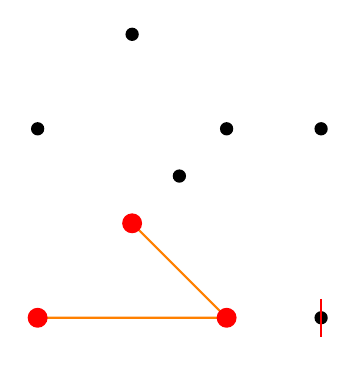
\begin{tikzpicture}[scale=1.2]
            % Points
            \foreach \x/\y/\n in {1/1/1, 3/1/3, 4/1/8, 2/2/2, 2.5/2.5/9, 3/3/7, 4/3/4, 2/4/5, 1/3/6} {
                \fill (\x,\y) circle (2pt);
            }
            % Stack: p0, p3, p2 (backtrack: remove p8)
            \draw[thick, orange] (1,1) -- (3,1) -- (2,2);
            \fill[red] (1,1) circle (3pt);
            \fill[red] (3,1) circle (3pt);
            \fill[red] (2,2) circle (3pt);
            % Cross out p8
            \draw[red, thick] (4,1.2) -- (4,0.8);
        \end{tikzpicture}
        \caption{Step 4b: Backtrack (remove point)}
    \end{subfigure}
    \begin{subfigure}{0.32\textwidth}
        \centering
        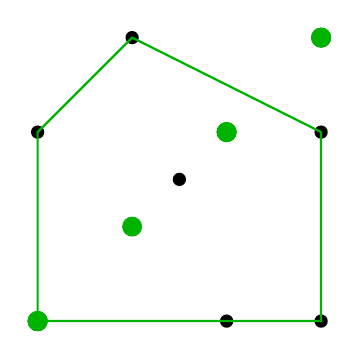
\begin{tikzpicture}[scale=1.2]
            % Points
            \foreach \x/\y/\n in {1/1/1, 3/1/3, 4/1/8, 2/2/2, 2.5/2.5/9, 3/3/7, 4/3/4, 2/4/5, 1/3/6} {
                \fill (\x,\y) circle (2pt);
            }
            % Final hull
            \draw[thick, green!70!black] (1,1) -- (3,1) -- (4,1) -- (4,3) -- (2,4) -- (1,3) -- (1,1);
            \foreach \x/\y in {1,1, 3,1, 4,1, 4,3, 2,4, 1,3} {
                \fill[green!70!black] (\x,\y) circle (3pt);
            }
        \end{tikzpicture}
        \caption{Step 4c: Final hull}
    \end{subfigure}
    \caption{Step-by-step illustration of Graham Scan}
\end{figure}
\end{visualexample}
